\documentclass{homework}

\title{Homework 2}

\DeclareMathOperator{\Cov}{Cov}
\DeclareMathOperator{\Var}{Var}
\DeclareMathOperator{\Corr}{Corr}

\begin{document}
    \maketitle    

    \section{Problem 1}
    Without loss of generality, assume that $t\geq s$.
    Then by the law of distributivity,
    \begin{align*}
        \Cov(B_t,B_s)&=\Cov(B_t-B_s+B_s,B_s)\\
                     &=\Cov(B_t-B_s,B_s)+\Cov(B_s,B_s)
    \end{align*} 
    Since Brownian motion has independent increments,
    we have that
    \[\Cov(B_t-B_s,B_s)=0\]
    Therefore
    \[\Cov(B_t,B_s)=\Var(B_s)=s\]
    i.e.,
    \[\Cov(B_t,B_s)=\min\{t,s\}\]
    in general.

    Hence
    \[\Corr(B_t,B_s)=\frac{\Cov(B_t,B_s)}{\sqrt{\Var(B_t)\Var(B_s)}}
    =\frac{\min\{t,s\}}{\sqrt{ts}}\]

    \section{Problem 2}
    Note that $E\left(B_t^2\right)=t$, so by definition of
    covariance,
    \begin{equation}
        \label{eq:cov def}
        E\left((B_t^2-t)(B_s^2-s)\right)=\Cov(B_t^2,B_s^2)
    \end{equation}
    Also note that
    \begin{equation}
        \label{eq:cov formula}
        \Cov(B_t^2,B_s^2)=E(B_t^2B_s^2)-E(B_t^2)\cdot E(B_s^2)
    \end{equation}

    So the key to these problems is calculating $E(B_t^2B_s^2)$,
    which can be obtained by law of total expectation. Therefore,
    we can start from $E(B_t^2B_s^2|\mathcal F_s)$, and without
    loss of generality, we assume that $s\leq t$.

    We have that
    \begin{align*}
        E\left.\left(B_t^2B_s^2\right|\mathcal F_s\right)
        &=B_s^2E\left.\left(B_t^2\right|\mathcal F_s\right)\\
    \end{align*}
    and
    \begin{align*}
        E\left.\left(B_t^2\right|\mathcal F_s\right)
        &=E\left.\left((B_t-B_s+B_s)^2\right|\mathcal F_s\right)\\
        &=E\left((B_t-B_s)^2|\mathcal F_s\right)
            +2E\big(B_s(B_t-B_s)|\mathcal F_s\big)
            +E\left.\left(B_s^2\right|\mathcal F_s\right)
    \end{align*}
    Since Brownian motion has independent increments, we have
    that
    \begin{align*}
    E\left.\left((B_t-B_s)^2\right|\mathcal F_s\right)
    &=E\left((B_t-B_s)^2\right)=t-s\\
    E\left.\left(B_s(B_t-B_s)\right|\mathcal F_s\right)&=B_sE(B_t-B_s)=0\\
    E\left.\left(B_s^2\right|\mathcal F_s\right)&=B_s^2
    \end{align*}
    Hence
    \begin{align*}
        E\left.\left(B_t^2B_s^2\right|\mathcal F_s\right)
        &=B_s^2\cdot E\left.\left(B_t^2\right|\mathcal F_s\right)\\
        &=B_s^2\left(t-s+B_s^2\right)
    \end{align*} 

    Therefore
    \begin{align*}
    E\left(B_t^2B_s^2\right)&=E\left(E\left.\left(B_t^2B_s^2\right|\mathcal F_s\right)\right)\\
    &=E\left(B_s^2\left(t-s+B_s^2\right)\right)\\
    &=(t-s)E\left(B_s^2\right)+E\left(B_s^4\right)
    \end{align*}


    As for $E\left(B_s^4\right)$, since that $\left(B_s/\sqrt{s}\right)^2
    \sim\chi^2(1)$, we obtain,
    \[\Var(B_s^2)=2s^2\]
    thus
    \begin{align*}
        E\left(B_s^4\right)&=\Var\left(B_s^2\right)+\left(E\left(B_s^2\right)\right)^2=3s^2
    \end{align*}
    It follows that
    \begin{align*}
    E\left(B_t^2B_s^2\right)=s(t+2s)
    \end{align*}
    so in general by symmetry,
    \begin{equation}
        \label{eq:EBs2Bt2}
        E\left(B_t^2B_s^2\right)=ts+2\min\{t,s\}
    \end{equation}

    \begin{subproblem}
        \item\label{pb:2.1}
        From \cref{eq:cov def,eq:cov formula} we know that
        \[E\left((B_t^2-t)(B_s^2-s)\right)=ts+2\min\{t,s\}-ts=2\min\{t,s\}\]

        \item
        As in \cref{eq:EBs2Bt2}
        \[E\left(B_t^2B_s^2\right)=ts+2\min\{t,s\}\]

        \item
        Same as \ref{pb:2.1} as shown by \cref{eq:cov def},
        \[\Cov(B_t^2,B_s^2)=2\min\{t,s\}\]
    \end{subproblem}

    \section{Problem 3}
    \begin{proof}
        Since $2X_i-1$ represents the movements of every step,
        we have that
        \[Y_n=\Delta x\cdot\left(\sum_{i=1}2X_i-1\right)
        =\Delta x(2S_n-n)\]
        Then by Laplace-De Moivre Theorem,
        \[\frac{S_n-\frac{n}{2}}{\sqrt{\frac{n}{4}}}\to N(0,1)\]
        i.e.,
        \[\frac{Y_n}{\sqrt{n}\Delta x}\to N(0,1)\]
        Since $D=(\Delta x)^2/\Delta t$ and $t=n\Delta t$,
        we have that
        \[\frac{Y_n}{\sqrt{n}\Delta x}=\frac{Y_n}{\sqrt{Dt}}\]
        And $n\to\infty$ is equivalent $t\to\infty$, therefore
        \[\frac{Y_t}{\sqrt{Dt}}\to N(0,1)\]
        It follows that
        \begin{align*}
        \lim_{n\to\infty,t=n\Delta t}P(a\leq Y_t\leq b)
        &=\frac{1}{\sqrt{2\pi}}
        \int_{a/\sqrt{Dt}}^{b/\sqrt{Dt}}\e^{-\frac{\xi^2}{2}}\diff\xi\\
        &=\frac{1}{\sqrt{2\pi Dt}}
        \int_a^b\e^{-\frac{x^2}{2Dt}}\diff x
        \end{align*}
    \end{proof}

    \section{Problem 4}
    \begin{subproblem}[\roman*)]
        \item
        Let's start from the high dimension directly.
        Denote random variable
        \[Z_i:=\begin{cases}
            W_{t_1},&i=1\\
            W_{t_i}-W_{t_{i-1}},&i>1
        \end{cases}\]
        By the independent increments of Brownian motion, we
        obtain $Z_i,i=1,2,\ldots,N$ are mutually independent.
        Then the joint distribution of $(Z_1,Z_2,\ldots,Z_N)$
        is clear and simple -- we have the JPDF
        \begin{equation*}
            p(z_1,z_2,\ldots,z_N)=
            \frac{\e^{-\frac{1}{2}\left(
                \frac{z_1^2}{t_1}
                +\frac{z_2^2}{t_2-t_1}
                +\cdots+\frac{z_N^2}{t_N-t_{N-1}}
            \right)}}{\sqrt{(2\pi)^Nt_1(t_2-t_1)\cdots(t_N-t_{N-1})}}
        \end{equation*}

        For the event $\{\omega;a_i\leq W_{t_i}(\omega)\leq b_i\}$,
        it is equivalent to
        \[\left\{\omega;a_i\leq \sum_{k=1}^iZ_k(\omega)\leq b_i\right\}\]
        It follows that
        \begin{equation}
            \label{eq:p4 mult-integral}
            \begin{aligned}
            &P(\omega;a_i\leq W_{t_i}\leq b_i,i=1,2,\ldots,N)\\
            =&P\left(\omega;a_i\leq \sum_{k=1}^iZ_k(\omega)\leq b_i,i=1,2,\ldots,N\right)\\
            =&\int_{\left\{z\in\mathbb R^N;a_i\leq\sum_{k=1}^iz_i\leq b_i,i=1,2,\ldots,N\right\}}
              p(z_1,z_2,\ldots,z_N)
              \diff z_1\diff z_2\cdots\diff z_N
            \end{aligned}
        \end{equation}
        Then by variable subtitution of the following,
        \begin{align*}
            z_1&=w_1,\\
            z_i&=w_i-w_{i-1},i=2,3,\ldots,N\\
        \end{align*}
        we have the Jacobian determinant
        \[\mathcal J=
        \frac{\partial(z_1,z_2,\ldots,z_N)}{\partial(w_1,w_2,\ldots,w_N)}
        =\det\begin{pmatrix}
            1  &        &        &       \\
            -1 & 1      &        &       \\
               & \ddots & \ddots &       \\
               &        & -1     & 1     \\
        \end{pmatrix}=1\]
        thus \cref{eq:p4 mult-integral} becomes
        \begin{align*}
            &P(\omega;a_i\leq W_{t_i}\leq b_i,i=1,2,\ldots,N)\\
            =&\int_{\prod_{i=1}^N[a_i,b_i]}
              p(w_1,w_2-w_1,\ldots,w_N-w_{N-1})
              |\mathcal J|
              \diff w_1\diff w_2\cdots\diff w_N\\
            =&\int_{\prod_{i=1}^N[a_i,b_i]}
               \frac{\e^{-\frac{1}{2}\left(
                   \frac{w_1^2}{t_1} 
                   +\frac{(w_2-w_1)^2}{t_2-t_1}
                   +\cdots
                   +\frac{(w_N-w_{N-1})^2}{t_N-t_{N-1}}
               \right)}}{\sqrt{(2\pi)^Nt_1(t_2-t_1)\cdots(t_N-t_{N-1})}}
              \diff w_1\diff w_2\cdots\diff w_N\\
        \end{align*}

        \item
        As $N\to\infty$, there are infinitely many $W_{t_i}\in[a,b]$,
        which should be rarely happening. So in conclusion,
        \[\lim_{N\to\infty}P\left(
            \omega;
            a_i\leq W_{t_i}\leq b_i,
            \forall i=1,2,\ldots,N
        \right)=0\]
        
        \item
        As \sidenote{Since the work of calculation increases rapidly
        as $N$ increases, only a few $N$s is chosen.}
        \cref{fig:integral}.
        \begin{marginfigure}
            \centering
            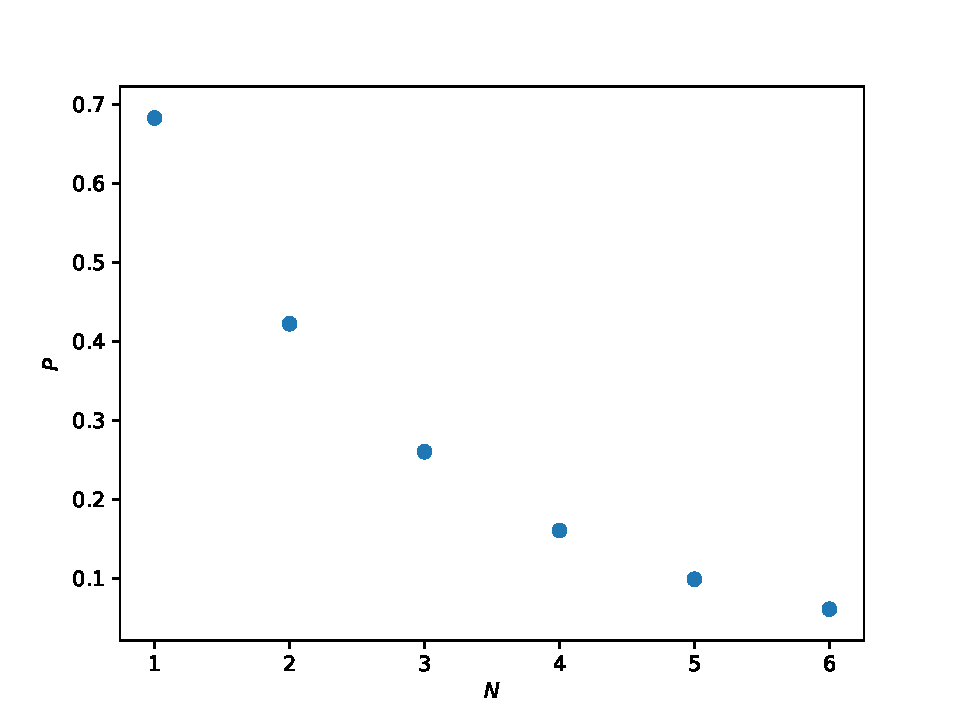
\includegraphics[width=\columnwidth]{integral}
            \caption{Approximation as $N\to\infty$}
            \label{fig:integral}
        \end{marginfigure}
    \end{subproblem}
\end{document}